\section{Resultados}
% NOTE:
% You are expected to refer to all the floats (figures, tables, etc.)
% in the results section.
Para los resultados fue necesario recolectar dentro un TXT los datos obtenidos que eran necesarios para el análisis de complejidad. Dentro de este TXT de resultados se presentan 3 columnas. La primera columna hace referencia a la cantidad de números que se encuentran dentro del TXT que estamos leyendo. La segunda columna hace referencia a la cantidad de comparaciones realizadas durante todo el algoritmo y finalmente la tercera columna hace referencia al tiempo que se demoró el algoritmo en realizar todo el trabajo solicitado. Los resultados del experimento son los siguientes:\\

% shows how to create a table and how to refer to it

\begin{table}[H]	% uses float package to control placement
	\centering	% centers the table
	\caption{
		Resultados obtenidos y almacenados en el archivo TXT
	}	% provides a concise description of the table contents

	\begin{tabular}{r r r}
		% table header
		Tamaño & Operaciones & Tiempo transcurrido \\ 
		% inserts horizontal line
		\hline 
		% separates column entries with the ampersand &
		1000 & 3995 &  331491 \\
		1500 & 4661 &  129010 \\
		2250& 8267 &  356851 \\
		3375& 11444 & 230468 \\
		5062& 17134&  349452 \\
	    7593 & 28501 & 775948 \\
	    11389 & 36493 & 764596 \\
	    17083 & 65561 & 1147673 \\
	    25624 & 82791 & 1630712 \\
	    38436 & 135055 & 2382282 \\
	    57654 & 207684 & 4084460 \\
	    86481 & 283434 & 5366096 \\
	    129721 & 510508 & 9863766 \\
	    194581 & 604273 & 12823640 \\
	    291871 & 1064734 & 18091307 \\
	    437806 & 1505635 & 31811224 \\
	    656709 & 2208375 & 46339697 \\
	    985063 & 3732436 & 83669467 \\
	        
	\end{tabular}

	% defines a label to refer to it
\end{table}

La gráfica obtenida con estos datos es la siguiente:

\begin{figure}[H]
	% centers the figure
	\centering
	% my LaTeX installation expects Encapsulated PostScript EPS graphs
	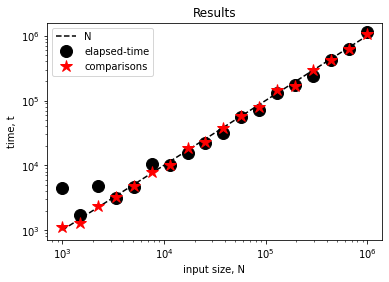
\includegraphics[keepaspectratio, width = 0.75\textwidth]{Graphic.png}
	\caption{
	  Número promedio de operaciones y tiempo de ejecución como función del tamaño del set de coordenadas.  
	}
	% defines a label to refer to it
	\label{fig:best}
\end{figure}
Como se puede observar en la gráfica, el comportamiento de los datos es claramente lineal. La línea punteada representa el comportamiento esperado para el experimento, el cuál es líneal. Los resultados obtenidos siguen el comportamiento esperado, puesto que la pendiente también corresponde a un comportamiento lineal. Los primeros datos de tiempo transcurrido difieren de lo esperado, pero estos no representan el comportamiento real del algoritmo puesto que son solo 3 datos atípicos que se deben a que las primeras ejecuciones pueden tardar más de lo esperado en lo que se normaliza su comportamiento. Otra observación importante es que algunos puntos se encuentran ligeramente por debajo o por encima de la pendiente. Esto puede deberse a que la lista de posibles candidatos es la que mayor complejidad y tiempo de ejecución añade al algoritmo puesto que utiliza la función de búsqueda por fuerza bruta a todos los candidatos que pueden ser muchos más de 3. De esta forma, si la lista de candidatos es muy grande el tiempo que se tarda en completar la tarea puede aumentar y viceversa. Esto podría ser una posible explicación para dicha variación. Aparte de esto, es evidente que la complejidad del algoritmo es de O(n) tal y como se esperaba. 

Ahora bien, la complejidad del algortimo resulta O(n) debido a que se usa la recursividad. Al dividirse el set de datos en subsets de tamaño 3 o menor, la complejidad para hallar el par de puntos más cercanos de un grupo de 3 es baja. La verdadera complejidad del algoritmo se encuentra en la búsqueda de candidatos y la subsequente aplicación de Fuerza Bruta en este set de candidatos. La complejidad para cada operación es de O(n). Por tanto, el resultado de la complejidad sería algo como T(n) = 2T(n/2) + O(n) + O(n) = 2T(n/2) + 2 O(n). Esto claramente da como resultado una complejidad lineal de O(n).



